温度$T_b=0$℃、一定の無限平板(厚さ 20 \si{\cm})の片側表面を急に$T_a = 1000$℃にした場合の温度変化に関して、
後退差分法のトーマス法による数値解析をソースコード\ref{s1}に示す。時間ステップは250 \si{s}、解析結果を1000 \si{s}ごとに5000 \si{s}
ごとに出力したものを図\ref{im1}に示す。
\begin{lstlisting}[caption=後退差分法のトーマス法による数値解析プログラム,label=s1]
#include<stdio.h>

#define N 10        // メッシュ数
#define L 0.2       // 棒の長さ
#define dx (L / N)  // メッシュの間隔
#define T0 1000     // 左端の温度
#define T1 0        // 右端の温度
#define dt 250      // 時間刻み幅
  
int T_final = 5000; // 解析終了時間
double alpha = 1.26/(1600*1050);// 熱伝達率
double T_old[N+1];  // 未知数の温度分布
double T_new[N+1];  // 次の時間ステップの温度分布
double a[N-1];      // トーマス法の行列の係数a~d
double b[N-1]; 
double c[N-1]; 
double d[N-1]; 
double r = (alpha*dt/(dx*dx)); //収束判定
  
void ThomasAlgorithm(){
  
  // 時間ステップごとの反復
  int t = 250;
  while(t <= T_final){
    //トーマス法の計算
    for(int x = 1; x < N-1; x++){
      double e = a[x]/b[x-1];
      b[x] = b[x] - e * c[x-1];
      d[x] = d[x] - e * d[x-1];
    }
    d[N-2] = d[N-2]/b[N-2];
    for(int x = N - 3; x >= 0; x--){
      d[x] = (d[x] - c[x] * d[x+1])/b[x];
    }
    for(int x = 1; x < N; x++){
      T_new[x] = d[x-1];
    }
    //1000秒ごとに表示
    if(t % 1000 == 0){
      printf("%d[s] ",t);
      for(int x = 0; x < N+1; x++){
        printf("%5.1f\t",T_new[x]);
      }
      printf("\n");
    } 
    for(int x = 0; x < N+1; x++){
      T_old[x] = T_new[x];
    }
    for(int x = 0; x < N-1; x++){
      a[x] = -r;
      b[x] = 1 + 2 * r;
      c[x] = -r;
      if(x == 0){
      d[x] = r * T_old[x] + T_old[x+1]; 
      }else if(x == N - 2){
        d[x] = r * T_old[x+2] + T_old[x+1]; 
      }else{
        d[x] = T_old[x+1];
      }
    }
    t+=dt;
  }
}
  
int main(){
      //境界条件
  for(int x = 1; x < N; x++){
    T_old[x] = T1;
    T_new[x] = T1;  // 初期温度分布を0℃で初期化
  }
  T_old[0] = T0;
  T_new[0] = T0;
  
  for(int x = 0; x < N-1; x++){
    a[x] = -r;
    b[x] = 1 + 2 * r;
    c[x] = -r;
    if(x == 0){
      d[x] = r * T_old[x] + T_old[x+1]; 
    }else if(x == N - 2){
      d[x] = r * T_old[x+2] + T_old[x+1]; 
    }else{
      d[x] = T_old[x+1];
    }
  }
  ThomasAlgorithm();
  return 0;
}
\end{lstlisting}

\begin{figure}[H]
  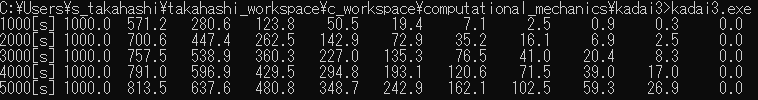
\includegraphics[width=\columnwidth]{img/k3.png}
  \caption{実行結果}
  \label{im1}
\end{figure}